%%%%%%%%%%%%%%%%%%%% CHAPTER 3 %%%%%%%%%%%%%%%%%%%%%%%%%%
%%%%% Variables and Operators %%%%%%%%%%%%%%%%%%%%%%%%%%%%%%%%%%% 
\section{Sorting}
Another frequent task in engineering hydraulics is the seemingly mundane task of sorting or ordering things. 
Here we explore a couple of simple sorting algorithms, just to show some of the thoughts that go into such a task, then will ultimately resort to the internal sorting routines built into R.
\subsection{Bubble Sort}
The bubble sort is a place to start despite it's relative slowness.
It is a pretty reviled algorithm (read the Wikipedia entry), but it is the algorithm that a naive programmer might cobble together in a hurry, and despite its shortcomings (its really slow and inefficient), it is robust.

Here is a description of the sorting task as described by \cite{Christian2016} (pg. 65):
\begin{quote}
``Imagine you want to alphabetize your unsorted collection of books. A natural approach would be just to scan across the shelf looking for out-of-order pairs -- Wallace followed by Pynchon, for instance -- and flipping them around. Put Pynchon ahead of Wallace, then continue your scan, looping around to the beginning of the shelf each time you reach the end. When you make a complete pass without finding any more out-of-order pairs on the entire shelf, then you know the job is done.

This process is a Bubble Sort, and it lands us in quadratic time. There are $n$ books out of order, and each scan through the shelf can move each one at most one position. (We spot a tiny problem, make a tiny fix.) So in the worst case, where the shelf is perfectly backward, at least one book will need to be moved n positions. Thus a maximum of $n$ passes through $n$ books, which gives us $O(n2)$ in the worst case.\footnote{Actually, the average running time for Bubble Sort isn't any better, as books will, on average, be $n/2$ positions away from where they?re supposed to end up. One would round the $n/2$ passes of $n$ books up to $O(n2)$.}
$\dots \dots$  For instance, it means that sorting five shelves of books will take not five times as long as sorting a single shelf, but twenty-five times as long.''
\end{quote}

Converting the word description into \textbf{R} is fairly simple.  We will have a vector of $n$ numbers (we use a vector because its easy to step through the different positions), and we will scan through the vector once (and essentially find the smallest thing), and put it into the first position.  Then we scan again from the second position and find the smallest thing remaining, and put it into the second position, and so on until the last scan which should have the remaining largest thing.  If we desire a decreasing order, simply change the sense of the comparison.  

Listing \ref{lst:MyBubbleSort.R} is an \textbf{R} script that implements the algorithm -- in the script the actual sort is treated as a function (we may actually want to use it again someday) which is loaded into the programming environment first, then an array is defined, and sorted.  The program (outside of the sorting algorithm) is really quite simple.  
\begin{itemize}
\item Load the sorting function.
\item Load contents into an array to be sorted.
\item Echo (print) the array (so we can verify the data are loaded as anticipated).
\item Sort the array, put the results back into the array (an in-place sort).
\item Report the results.
\end{itemize}

\begin{lstlisting}[caption=R code demonstrating the naive bubble sort, label=lst:MyBubbleSort.R]
##############################################################
rm(list=ls())  # clear the object list (i.e. deallocate and clear memory)
### Bubble Sort Function -- Needs to be defined before sending array to sort ###
# Bubble Sort Function
# MyLocation: ~/Dropbox/1-CE-TTU-Classes/CE4333-PCH-R/1-Lectures/Lecture03/ScriptsInLecture
# Bubble Sort with array indexing starting at [1] 
# Compare to Python or C where arrays start at [0])
# by: Theodore G. Cleveland 2017-0317
################################################################
bubble <- function(array)
{
  # Prepare the sort, need to know how many things and need a temporary store
  swap <- numeric(0) # temporary store (aka swap location)
  howMany <- length(array) # how many things to be sorted
  # The actual sorting process
  for (irow in 1:(howMany-1))
  {
    for (jrow in 1:(howMany-irow))
    {
      if( array[jrow] > array[jrow+1])
      {
        swap <- array[jrow];
        array[jrow] <- array[jrow+1];
        array[jrow+1] <- swap;
      }
    } 
  }
  # return result (sort in-place)
  return(array)
}
##############################################################

##############################################################
xarray <- c(1003,3.2,55.5,-0.0001,-6,666.6,102)  # the array to sort
print(xarray)
xarray <- bubble(xarray)
print(xarray)
##############################################################
\end{lstlisting}  

Figure \ref{fig:MyBubbleSort.jpg} is a screen capture of the script running.   
In the figure we see that the program (near the bottom of the file) assigns the values to the vector named array and the initial order of the array is $[1003,3.2,55.5,-0.0001,-6,666.6,102]$.   
The smallest value in the example is $-6$ and it appears in the 5-th position, not the 1-st as it should.  

The first pass through the array will move the largest value, $1003$, in sequence to the right until it occupies the last position.
Repeated passes through the array move the remaining largest values to the right until the array is ordered.  
One can consider the values of the array at each scan of the array as a series of transformations (\texttt{irow}-th scan) -- in practical cases we don't necessarily care about the intermediate values, but here because the size is manageable and we are trying to get our feet wet with algorithms, we can look at the values.

The sequence of results (transformations) after each pass through the array is shown in the following list:
\begin{enumerate}
\item Initial value: $[1003,3.2,55.5,-0.0001,-6,666.6,102]$.
\item First pass: $[3.2,55.5,-0.0001,-6,666.6,102,1003]$.
\item Second pass: $[3.2,-0.0001,-6,55.5,102,666.6,1003]$.
\item Third pass: $[-0.0001,-6,3.2,55.5,102,666.6,1003]$.
\item Fourth pass: $[-6,-0.0001,3.2,55.5,102,666.6,1003]$.
\item Fifth pass:  $[-6,-0.0001,3.2,55.5,102,666.6,1003]$. Sorted, fast scan.
\item Sixth pass: $[-6,-0.0001,3.2, 55.5,102,666.6,1003]$.  Sorted, fast scan.
\end{enumerate}
\begin{figure}[h!] %  figure placement: here, top, bottom, or page
   \centering
   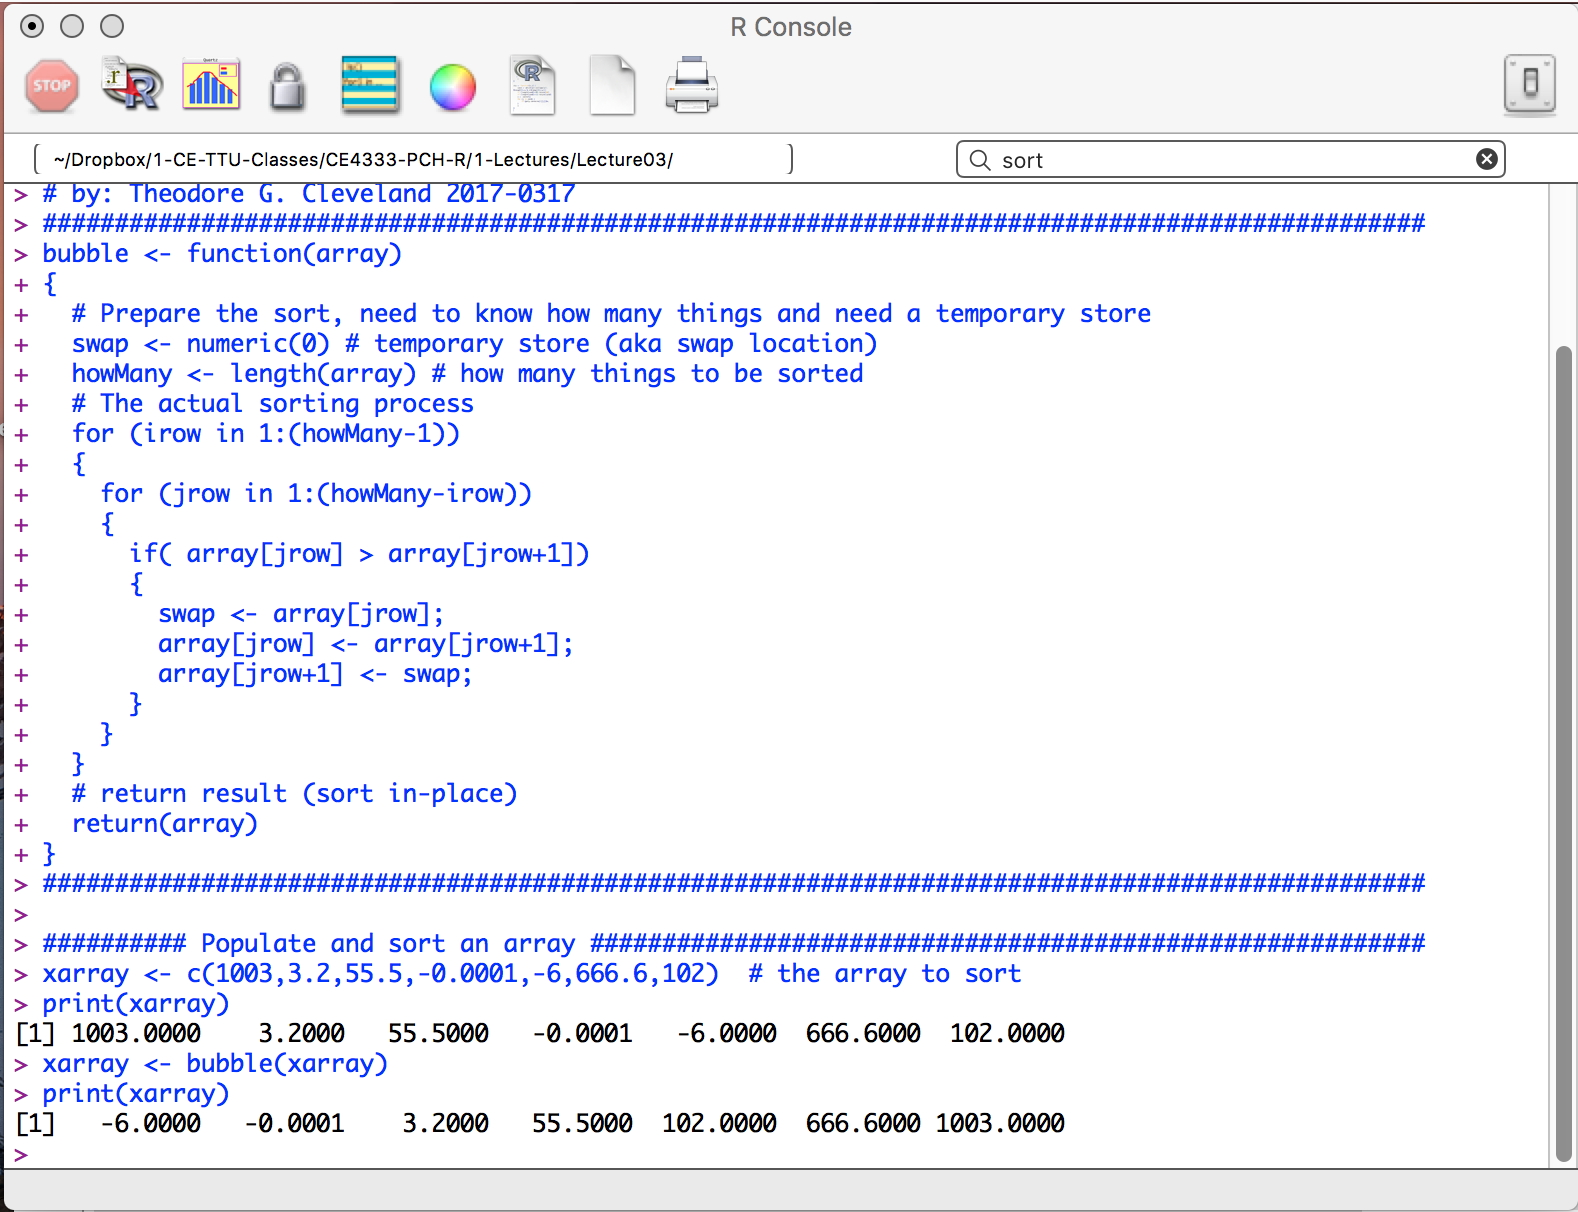
\includegraphics[width=6in]{./3-Sorting/MyBubbleSort.jpg} 
   \caption{Bubble Sort implemented in \textbf{R}}
   \label{fig:MyBubbleSort.jpg}
\end{figure}

We could probably add additional code to break from the scans when we have a single pass with no exchanges -- while meaningless in this example, for larger collections of things, being able to break out when the sorting is complete is a nice feature.
\clearpage

\subsection{Insertion Sort}
The next type of sorting would be to select one item and locate it either left or right of an adjacent item based on its size -- like sorting a deck of cards, or perhaps a better description -- again using the bookshelf analog from \cite{Christian2016} (pg. 65):
\begin{quote}
``$\dots \dots$ You might take a different tack -- pulling all the books off the shelf and putting them back in place one by one. You'd put the first book in the middle of the shelf, then take the second and compare it to the first, inserting it either to the right or to the left. Picking up the third book, you'd run through the books on the shelf from left to right until you found the right spot to tuck it in. Repeating this process, gradually all of the books would end up sorted on the shelf and you'd be done. Computer scientists call this, appropriately enough, Insertion Sort. The good news is that it's arguably even more intuitive than Bubble Sort and doesn't have quite the bad reputation. The bad news is that it's not actually that much faster. You still have to do one insertion for each book. And each insertion still involves moving past about half the books on the shelf, on average, to find the correct place.

Although in practice Insertion Sort does run a bit faster than Bubble Sort, again we land squarely, if you will, in quadratic time. Sorting anything more than a single bookshelf is still an unwieldy prospect.''
\end{quote}

Listing \ref{lst:MyInsertionSort.R} is an \textbf{R} implementation of a straight insertion sort.  
The script is quite compact, and I used indentation and extra line spacing to keep track of the scoping delimiters.
The sort works as follows, take the an element of the array (start with 2 and work to the right) and put it into a temporary location (called \texttt{swap} in my script).  Then compare locations to the left of \texttt{swap}.  If smaller, then break from the loop, exchange values, otherwise the values are currently ordered. Repeat (starting at the next element) , when all elements have been traversed the resulting vector is sorted.  Here are the transformations for each pass through the outer loop:
\begin{enumerate}
\item Pass 0: $[1003,3.2,55.5,-0.0001,-6,666.6,102]$, Initial array.
\item Pass 1: $[3.2,1003,55.5,-0.0001,-6.,666.6,102]$.
\item Pass 2: $[3.2,55.5,1003,-0.0001,-6.,666.6,102]$.
\item Pass 3: $[-0.0001,3.2,55.5,1003,-6.,666.6,102]$.
\item Pass 4: $[-6,-0.0001,3.2,55.5,1003.,666.6,102]$.
\item Pass 5: $[-6,-0.0001,3.2,55.5,666.6,1003,102]$.
\item Pass 6: $[-6,-0.0001,3.2,55.5,102,666.6,1003]$, Sorted array.
\end{enumerate}
Figure \ref{fig:MyInsertionSort.jpg} is a screen capture of the insertion sort in operation.  
Insertion sorting is reasonably fast for small lists (about 50 or so elements) and forms the basis of the internal sorts in other routines that divide up the overall list into smaller lists, sort the smaller lists, then uses a merge to collate back to the overall list (now sorted).
\begin{lstlisting}[caption=R code demonstrating the insertion sort, label=lst:MyInsertionSort.R]
### Straight Insertion Sort Function by: Theodore G. Cleveland 2017-0317
rm(list=ls())  # clear the object list (i.e. deallocate and clear memory)
################################################################
insertSort <- function(array){
# Prepare the sort, need to know how many things and need a temporary store
  swap <- numeric(0) # temporary store (aka swap location)
  howMany <- length(array) # how many things to be sorted
  for (j in 2:howMany)  # select each position in turn
    {
    test <- 0           # set a test value, used to insert later
    swap <- array[j]    # current position to swap
    for (i in seq(j-1,1,by=-1)) #find place to insert by ...
      {
      if (array[i] <= swap)  # test if current position is bigger
        {
        test <- 1            # if true set test to 1, break inner loop
        break
        }
      array[i+1] <- array[i]  # otherwise exchange postions
      }
    if(test == 1)             # if broke from loop, insert swap
      array[i+1] <- swap      
    else
      i = 0
      array[i+1] <- swap      # otherwise swap goes to first position
    }
  return(array) }    # return result (sort in-place)
##############################################################
xarray <- c(1003,3.2,55.5,-0.0001,-6,666.6,102)  # the array to sort
print(xarray)
xarray <- insertSort(xarray)
print(xarray)
##############################################################
\end{lstlisting}  


\begin{figure}[h!] %  figure placement: here, top, bottom, or page
   \centering
   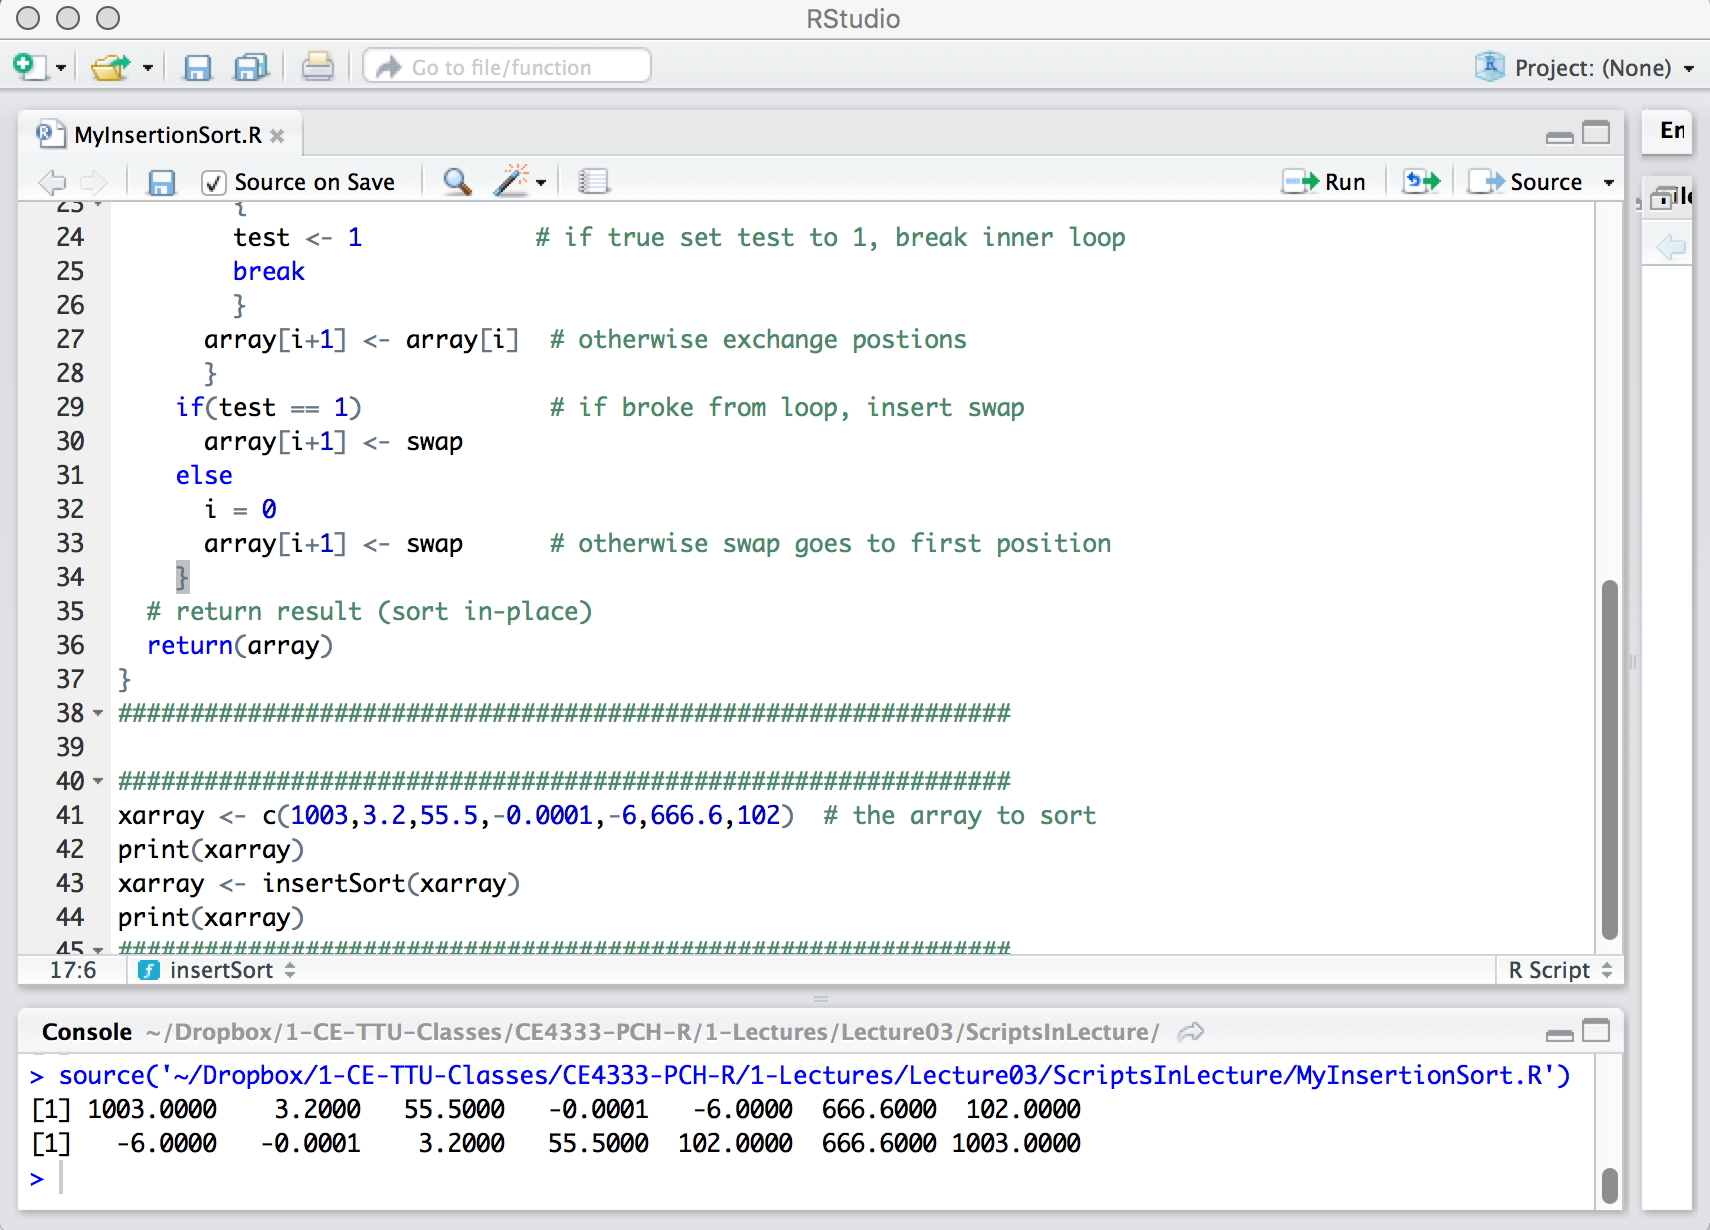
\includegraphics[height=4.2in]{./3-Sorting/MyInsertionSort.jpg} 
   \caption{Insertion Sort implemented in \textbf{R}}
   \label{fig:MyInsertionSort.jpg}
\end{figure}

\subsection{Merge Sort}
A practical extension of these slow sorts is called the Merge Sort.  It is an incredibly useful method.  One simply breaks up the items into smaller arrays, sorts those arrays - then merges the sub-arrays into larger arrays (now already sorted), and finally merges the last two arrays into the final, single, sorted array.

Here is a better description, again from \cite{Christian2016}:
\begin{quote}
``$\dots \dots$ information processing began in the US censuses of the nineteenth century, with the development, by Herman Hollerith and later by IBM, of physical punch-card sorting devices. In 1936, IBM began producing a line of machines called ``collators'' that could merge two separately \textbf{ordered} stacks of cards into one. \textit{As long as the two stacks were themselves sorted}, the procedure of merging them into a single sorted stack was incredibly straightforward and took linear time: simply compare the two top cards to each other, move the smaller of them to the new stack you're creating, and repeat until finished.

The program that John von Neumann wrote in 1945 to demonstrate the power of the stored-program computer took the idea of collating to its beautiful and ultimate conclusion. Sorting two cards is simple: just put the smaller one on top. And given a pair of two-card stacks, both of them sorted, you can easily collate them into an ordered stack of four. Repeating this trick a few times, you'd build bigger and bigger stacks, each one of them already sorted. Soon enough, you could collate yourself a perfectly sorted full deck -- with a final climactic merge, like a riffle shuffle's order-creating twin, producing the desired result. This approach is known today as Merge Sort, one of the legendary algorithms in computer science.''
\end{quote}

There are several other variants related to Merge Sort; Quicksort and Heapsort being relatives.  The creation of a Merge Sort is left to the reader if there is a need, and at this point we can just use the built-in \texttt{sort()}  and/or \texttt{order()} functions in \textbf{R} -- which implements either a Shellsort (useful if character strings are to be sorted) or Quicksort (used if numeric values are supplied).   We also have to supply if we want increasing or decreasing sorts.

Figure \ref{fig:BuiltInRSorts.jpg} illustrates using the built-in functions.  
For an ordinary sort, we simply use the function name \texttt{sort()} and direct its output into an object (it can even be the same vector as shown in the figure). 

If we wish to sort several related columns, based on values in one of the columns, it is easiest to construct a data frame (like a matrix), then order the contents based on one of the columns, and send the results to another data frame, or we can send the result back to itself.  Usually when we are manipulating multiple columns, we are operating in a ``relational database'' kind of mindset, and it is probably to our benefit to not destroy the original association structure.  Be aware of the syntax of a dataframe function, you will notice there is a comma that appears at the end of the function that is important for the script to function.

For example, \texttt{z <- z[order(xarray),]} will function as shown, \\ whereas \texttt{zztop <- z[order(xarray)]} will not.

\begin{figure}[h!] %  figure placement: here, top, bottom, or page
   \centering
   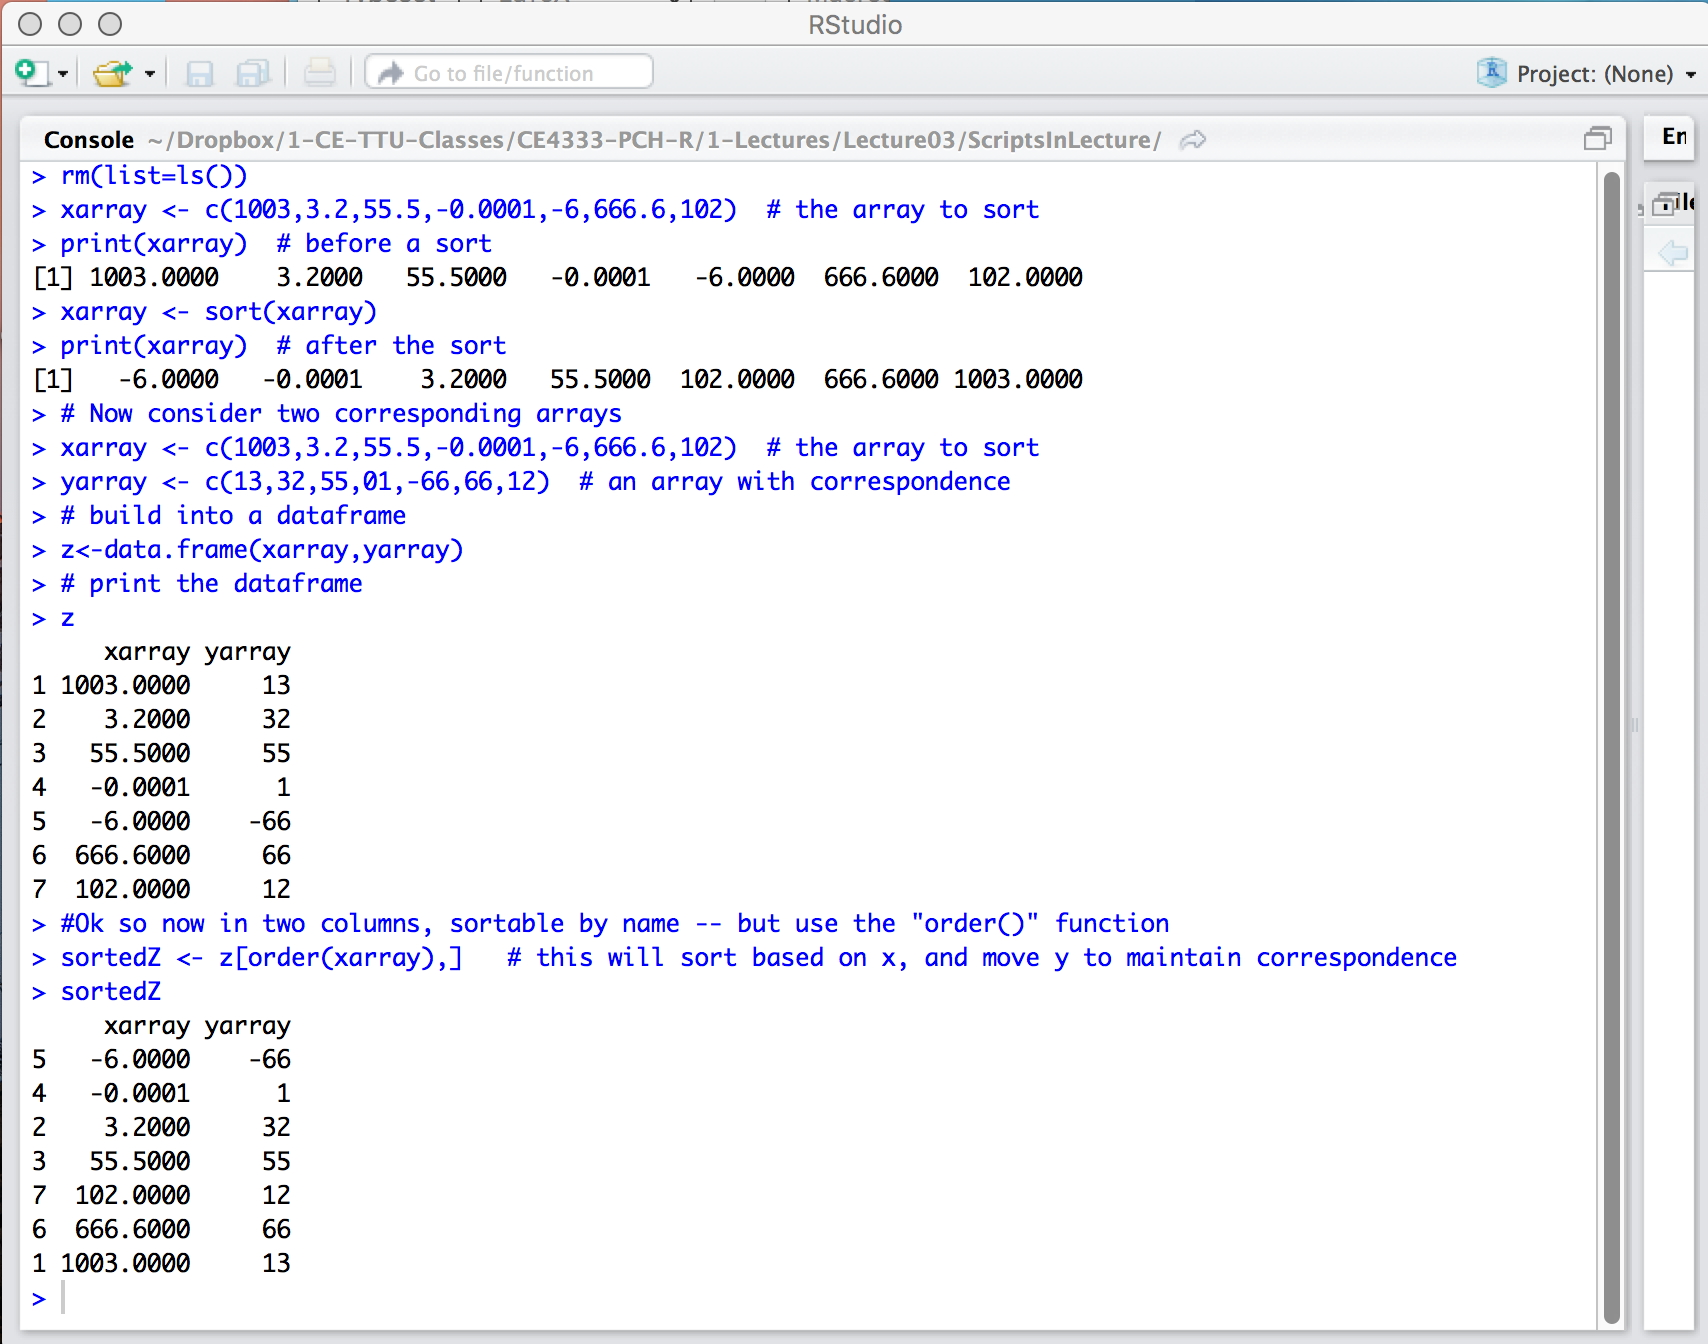
\includegraphics[width=6in]{./3-Sorting/BuiltInRSorts.jpg} 
   \caption{Sorting using built-in \textbf{R} functions}
   \label{fig:BuiltInRSorts.jpg}
\end{figure}

Now if we return to the interpolation chapter just before this one, we can immediately see a need for sorting.  The interpolation algorithm \textit{assumes} that the explanatory structure (x-axis) is ordered, otherwise the interpolation equation will return garbage.


I conclude this chapter with one more quoted section from \cite{Christian2016} about the value for sorting -- which is already relevant to a lot of computational hydraulics:
\begin{quote}
``The poster child for the advantages of sorting would be an Internet search engine like Google. It seems staggering to think that Google can take the search phrase you typed in and scour the entire Internet for it in less than half a second. Well, it can't -- but it doesn't need to. If you're Google, you are almost certain that (a) your data will be searched, (b) it will be searched not just once but repeatedly, and (c) the time needed to sort is somehow ``less valuable'' than the time needed to search. (Here, sorting is done by machines ahead of time, before the results are needed, and searching is done by users for whom time is of the essence.) All of these factors point in favor of tremendous up-front sorting, which is indeed what Google and its fellow search engines do.''
\end{quote}




%%%%%%%%%%%%%%%%%%%%%%%%%%%%%%%%%%%%%%%%%%%%%%%%%%%%

\subsection{Exercises}
\begin{enumerate}
\item Imagine you have two arrays, \texttt{array1} and \texttt{array2} that are linked in the sense that each element of \texttt{array1} is associated with the corresponding element of \texttt{array2}.  You wish to sort based on contents of \texttt{array1} and maintain the correspondence of \texttt{array2}.  In words we would simply modify the script to move and element of \texttt{array2} whenever you move an element of \texttt{array1}.

Modify the Insertion Sort script to accept two arrays, the sort is based on contents of the first array and you are to maintain correspondence with the second array.

Test your script on the following arrays:\\
\texttt{array1} = $[5,6,8,2,3,4,1]$\\
\texttt{array2} = $[24,35,63,3,8,15,0]$\\

when these are reordered, the result should be: \\
\texttt{array1} = $[1,2,3,4,5,6,8]$\\
\texttt{array2} = $[0,3,8,15,35,63]$\\

Then modify your script to read input from an ASCII file that contains the two arrays as columns (like in a spreadsheet) where you will sort on the first column, and carry along the correspondence with the second column.

Apply the script on the file \texttt{es3-pr1.txt}.

\item Repeat the exercise above but use built-in \textbf{R} functions.\footnote{My solution uses the \texttt{data.frame()} and \texttt{order()} functions.  There are probably several other ways to accomplish the goal -- corresponding sorts are hugely important in many practical situations.}   
\end{enumerate}


